\chapter{Processus de Poisson}
\sloppy


\section{Introduction et Motivation}
Nous voulons modéliser des événements qui arrivent à des dates précises mais imprévisibles.
\begin{example}
Exemples de tels événements incluent les séismes, la désintégration d'atomes, la pluie, ou le début et la fin d'appels téléphoniques.
\end{example}
À chaque occurrence d'un événement, nous marquons un impact sur l'axe des temps.
\begin{figure}[H]
\centering
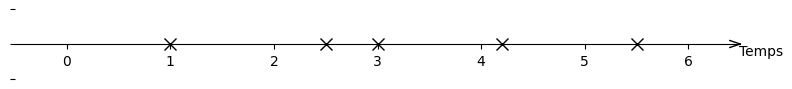
\includegraphics[width=0.8\textwidth]{time_axis_impacts.png}
\end{figure}
\section{Hypothèses du modèle}
Pour construire notre modèle, nous posons les hypothèses suivantes :
\begin{itemize}
    \item[i)] Les conditions de l'expérience ne changent pas au cours du temps.
    \item[ii)] Les nombres d'impacts dans des intervalles de temps disjoints sont indépendants.
\end{itemize}
Pour $t \ge 0$, nous notons $N(t)$ le nombre d'impacts dans l'intervalle $[0, t]$.
Nous avons ainsi une famille de variables aléatoires $(N(t))_{t \ge 0}$ indexée par un paramètre continu. C'est un \textbf{processus stochastique}.
\section{Construction d'un modèle discret}
Soit $n \ge 1$ un entier. Nous subdivisons l'axe réel en intervalles de longueur $\frac{1}{n}$, de la forme $\left[\frac{k}{n}, \frac{k+1}{n}\right[$, pour $k \ge 0$.
\begin{figure}[H]
\centering
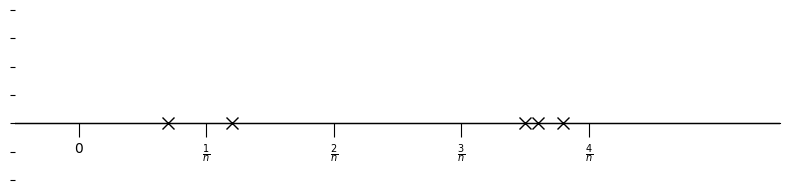
\includegraphics[width=0.8\textwidth]{discrete_time_axis.png}
\end{figure}
Un intervalle peut avoir $0, 1, 2, \dots$ impacts. 
\begin{definition}
Un intervalle $\left[\frac{k}{n}, \frac{k+1}{n}\right[$ est dit \textbf{occupé} s'il contient au moins un impact, et \textbf{vide} sinon.
\end{definition}
Notons $p_n$ la probabilité qu'un intervalle $\left[\frac{k}{n}, \frac{k+1}{n}\right[$ soit occupé. \\
D'après l'hypothèse (i), $p_n$ ne dépend pas de l'intervalle.\\
Pour $t>0$, notons $N_n(t)$ le nombre d'intervalles $\left[\frac{k}{n}, \frac{k+1}{n}\right[$ (avec $\frac{k+1}{n} \le t$) qui sont occupés.\\
Par l'hypothèse (ii), les états (vides ou occupés) de ces intervalles sont indépendants, et $N_n(t)$ suit la loi binomiale $B(\lfloor nt \rfloor, p_n)$.
\section{Convergence vers la loi de Poisson}
Nous étudions la limite en loi de $N_n(t)$, par exemple à l'aide des fonctions caractéristiques.
La fonction caractéristique de $N_n(t)$ est :
\[ \varphi_{N_n(t)}(u) = E[e^{iu N_n(t)}] = (1 - p_n + p_n e^{iu})^{\lfloor nt \rfloor} \]
Nous ajoutons une hypothèse supplémentaire : $p_n \to 0$ quand $n \to \infty$. Sinon, le modèle "explose".
Pour étudier la limite, nous analysons le logarithme de la fonction caractéristique :
\begin{align*}
\ln(\varphi_{N_n(t)}(u)) &= \lfloor nt \rfloor \ln(1 - p_n + p_n e^{iu}) \\
&= \lfloor nt \rfloor \ln(1 + p_n(e^{iu} - 1))
\end{align*}
En utilisant le développement limité $\ln(1+x) = x + o(x)$ pour $x \to 0$, on obtient :
\begin{align*}
\ln(\varphi_{N_n(t)}(u)) &= \lfloor nt \rfloor \left( p_n(e^{iu}-1) + o(p_n) \right) \\
&= \lfloor nt \rfloor p_n (e^{iu}-1) + o(n p_n)
\end{align*}
En passant à l'exponentielle :
\[ \varphi_{N_n(t)}(u) = e^{\lfloor nt \rfloor p_n (e^{iu}-1) + o(n p_n)} \]
Supposons que $np_n \to \lambda$ lorsque $n \to \infty$, où $\lambda$ est une constante positive. Alors $\lfloor nt \rfloor p_n \approx nt p_n \to \lambda t$.
La limite de la fonction caractéristique devient :
\[ \lim_{n \to \infty} \varphi_{N_n(t)}(u) = e^{\lambda t (e^{iu}-1)} \]
On reconnaît la fonction caractéristique d'une loi de Poisson de paramètre $\lambda t$.
Donc, $N_n(t)$ converge en loi vers une variable aléatoire suivant une loi de Poisson $\mathcal{P}(\lambda t)$.
\[ N_n(t) \xrightarrow{\mathcal{L}} \mathcal{P}(\lambda t) \]
\begin{remark}[Rappel sur la loi de Poisson]
Une variable aléatoire $X$ à valeurs dans $\mathbb{N}$ suit une loi de Poisson de paramètre $\lambda > 0$, notée $X \sim \mathcal{P}(\lambda)$, si pour tout $k \in \mathbb{N}$:
\[ P(X=k) = e^{-\lambda} \frac{\lambda^k}{k!} \]
Son \textbf{espérance} et sa \textbf{variance} sont égales à $\lambda$, i.e., $E[X] = \text{Var}[X] = \lambda$.\\
Sa \textbf{fonction caractéristique} est $\varphi_X(u) = \exp(\lambda(e^{iu}-1))$.
\end{remark}
\section{Instants de Saut}
Nous avons montré que, à $t$ fixé, $N_n(t) \xrightarrow{\mathcal{L}} \mathcal{P}(\lambda t)$.
Cependant, la fonction $t \mapsto N_n(t)$ est une \textbf{fonction aléatoire} en escalier, nulle en 0, croissante, et dont les accroissements sont soit 0, soit 1.
\begin{figure}[H]
\centering
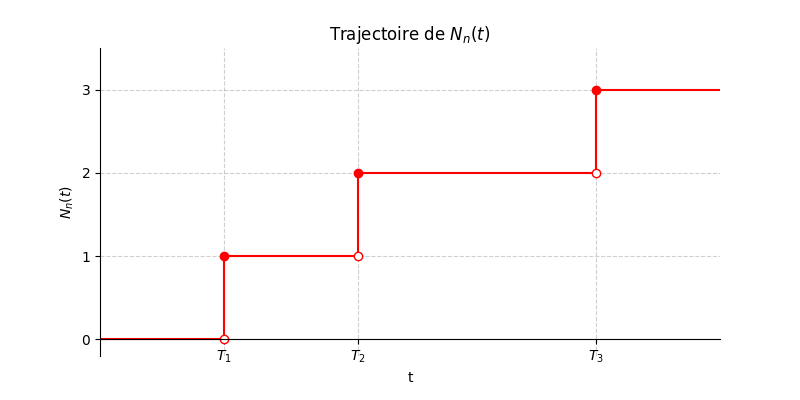
\includegraphics[width=0.8\textwidth]{Nn_t_plot.png}
\caption{Une réalisation de la fonction aléatoire $t \mapsto N_n(t)$.}
\end{figure}
La question se pose : la fonction aléatoire $t \mapsto N_n(t)$ converge-t-elle quand $n \to \infty$?
La fonction $N_n(t)$ est complètement déterminée par ses instants de saut. Nous définissons les instants de saut de $N_n(t)$ par :
\[ \forall k \ge 1, \quad T_k^n = \inf\left\{t \ge 0 : N_n(t)=k\right\} \]
En effet, on a $N_n(t) = \sum_{k=1}^\infty 1_{\{T_k^n \le t\}}$.
Examinons la convergence de ces instants de saut, en commençant par $T_1^n$.
Soit $i \ge 0$ un entier. L'événement $\{T_1^n > i/n\}$ signifie que les $i$ premiers intervalles de temps, $[0, 1/n), [1/n, 2/n), \dots, [(i-1)/n, i/n)$, sont tous vides.
Pour analyser cela, nous introduisons une suite de variables aléatoires $X_k$ pour $k \ge 0$ :
\[ X_k = \begin{cases} 0 & \text{si l'intervalle } [k/n, (k+1)/n[ \text{ est vide} \\ 1 & \text{sinon (occupé)} \end{cases} \]
Alors $P(T_1^n > i/n) = P(X_0=0, \dots, X_{i-1}=0)$. Par indépendance, ceci vaut $(1-p_n)^i$.
Pour $t>0$ fixé, choisissons $i = \lfloor nt \rfloor$. Alors :
\[ P(T_1^n > t) \approx P(T_1^n > \lfloor nt \rfloor / n) = (1-p_n)^{\lfloor nt \rfloor} \]
Comme nous avons supposé $np_n \to \lambda$, on a $p_n \approx \lambda/n$.
\[ P(T_1^n > t) \approx \left(1-\frac{\lambda}{n}\right)^{nt} \xrightarrow[n\to\infty]{} e^{-\lambda t} \]
On reconnaît la fonction de survie d'une loi exponentielle. Ainsi, $T_1^n \xrightarrow{\mathcal{L}} \text{Exp}(\lambda)$.
\begin{remark}[Rappel sur la loi Exponentielle]
Une variable aléatoire $X$ suit la loi exponentielle de paramètre $\lambda > 0$, notée $\text{Exp}(\lambda)$, si sa loi est de densité $f(x) = \lambda e^{-\lambda x}$ pour $x \ge 0$.
Son espérance est $E[X] = 1/\lambda$ et sa variance est $\text{Var}[X] = 1/\lambda^2$.
Sa fonction de répartition est $F_X(x) = P(X \le x) = 1 - e^{-\lambda x}$ pour $x \ge 0$.
\end{remark}
\begin{figure}[H]
    \centering
    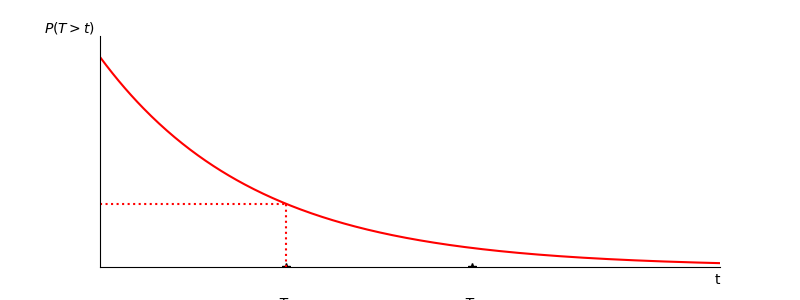
\includegraphics[width=0.7\textwidth]{exp_survival.png}
    \caption{Fonction de survie de la loi exponentielle.}
\end{figure}
On peut montrer de plus que les durées entre les sauts successifs sont indépendantes et de même loi.
Par exemple, $T_2^n - T_1^n$ est indépendant de $T_1^n$ et converge aussi en loi vers $\text{Exp}(\lambda)$.
Vérifions-le pour le modèle discret. 
\begin{remark}
Soient $i,j \ge 1$.\\
$$P(T_1^n = i/n, T_2^n - T_1^n = j/n) = P(X_0=0, \dots, X_{i-1}=0, X_i=1, X_{i+1}=0, \dots, X_{i+j-1}=0, X_{i+j}=1)$$.
Cette probabilité vaut $(1-p_n)^{i-1} p_n \cdot (1-p_n)^{j-1} p_n$.
Ceci est égal à $P(T_1^n = i/n) \cdot P(T_1^n = j/n)$. D'où le résultat.\\
Ainsi, le vecteur des inter-sauts converge en loi :
\[ (T_1^n, T_2^n - T_1^n, \dots, T_k^n - T_{k-1}^n) \xrightarrow[n\to\infty]{\mathcal{L}} (\text{Exp}(\lambda))^{\otimes k} \]
c'est-à-dire vers un vecteur de $k$ variables aléatoires indépendantes et de même loi $\text{Exp}(\lambda)$.
\end{remark}
\section{Le Processus de Poisson Continu}
Les calculs précédents nous permettent d'imaginer le candidat pour la limite en loi de $N_n(t)$.
\subsection{Définition à partir des instants de saut}
Soit $(Y_n)_{n \ge 1}$ une suite de variables aléatoires indépendantes et identiquement distribuées suivant la loi exponentielle $\text{Exp}(\lambda)$.
Posons $S_0=0$ et pour $n \ge 1$, $S_n = Y_1 + Y_2 + \dots + Y_n$.
La variable $S_n$ représente le temps du $n$-ième événement.
\begin{definition}[Processus de Poisson]
Pour tout $t \ge 0$, on définit le nombre d'événements jusqu'à l'instant $t$ par :
\[ N(t) = \max \{ n \ge 0 : S_n \le t \} \]
Le processus stochastique $(N(t))_{t \ge 0}$ est appelé le \textbf{processus de Poisson} d'intensité $\lambda$.
\end{definition}
\begin{figure}[H]
    \centering
    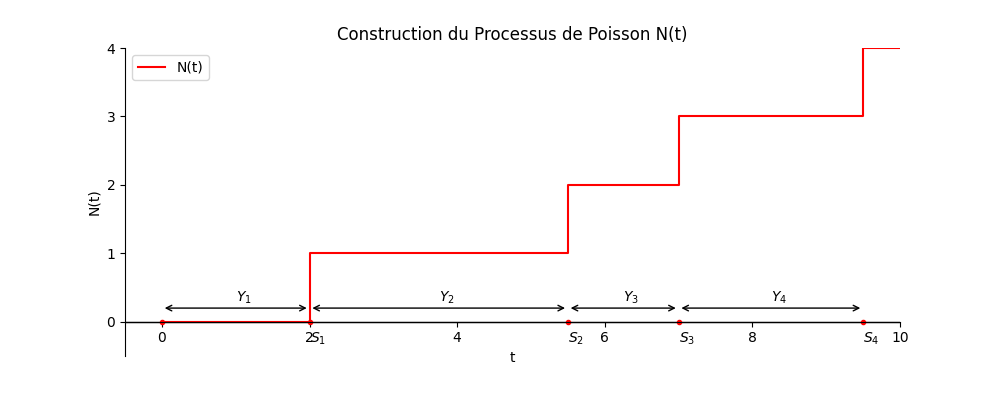
\includegraphics[width=\textwidth, keepaspectratio]{poisson_process_construction.png}
\end{figure}
Pour chaque $t$, $N(t)$ est une variable aléatoire qui suit une loi de Poisson $\mathcal{P}(\lambda t)$.
Nous avons ainsi construit un continuum de variables aléatoires $(N(t))_{t \ge 0}$ sur le même espace de probabilités.
On a $S_n \to +\infty$ presque sûrement. $N(t)$ est l'unique indice $k$ tel que $S_k \le t < S_{k+1}$.
\section{Applications}
\subsection{Application 1 : Bombardements de Londres (WWII)}
Pendant la Seconde Guerre mondiale, la ville de Londres a subi 537 impacts de bombes. La carte de la ville a été divisée en un quadrillage de 576 carrés de 0,25 km$^2$ chacun. Le nombre moyen d'impacts par carré est donc $\lambda = 537/576 \approx 0.9323$.
On compare le nombre de carrés ayant reçu $k$ impacts avec les prédictions de la loi de Poisson $\mathcal{P}(0.9323)$.
\begin{figure}[H]
    \centering
    
\includegraphics[width=0.4\textwidth]{london_grid.png}
    \caption{Quadrillage de la carte de Londres.}
\end{figure}
Le tableau suivant compare les données observées (nombre de carrés avec $k$ impacts) et les valeurs attendues selon la loi de Poisson ($576 \times P(X=k)$ avec $X \sim \mathcal{P}(0.9323)$).
\begin{center}
\begin{tabular}{|c|cccccc|}
\hline
\textbf{k (impacts)} & \textbf{0} & \textbf{1} & \textbf{2} & \textbf{3} & \textbf{4} & \textbf{$\ge 5$} \\
\hline
\textbf{Observé} & 229 & 211 & 93 & 35 & 7 & 1 \\
\textbf{Attendu} & 226.74 & 211.39 & 98.54 & 30.62 & 7.14 & 1.57 \\
\hline
\end{tabular}
\end{center}
\subsection{Application 2 : Problème d'Autobus}
Les arrivées de bus à un arrêt sont modélisées par un processus de Poisson d'intensité $\lambda$. Le temps moyen entre deux arrivées est donc $1/\lambda$.
J'arrive à l'instant $t$. Quel sera mon temps d'attente ?
\begin{figure}[H]
\centering
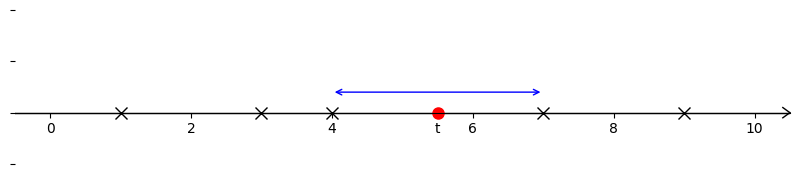
\includegraphics[width=\textwidth, keepaspectratio]{bus_arrival_timeline.png}
\end{figure}
\begin{itemize}
    \item \textbf{1er raisonnement :} Vu l'absence de mémoire de la loi exponentielle qui régit les temps entre les arrivées, mon temps d'attente suit une loi $\text{Exp}(\lambda)$, donc en moyenne $1/\lambda$.
    \item \textbf{2ème raisonnement :} J'arrive au hasard entre deux bus. Par symétrie, le temps moyen d'attente sera la moitié de la longueur typique des intervalles, soit $\frac{1}{2\lambda}$. Ce raisonnement est incorrect.
\end{itemize}
Soient $S_n = Y_1 + \dots + Y_n$ les instants d'arrivée des bus. Soit $k$ tel que $S_{k-1} < t \le S_k$.
Mon temps d'attente est $S_k - t$. L'erreur vient du fait que l'intervalle $[S_{k-1}, S_k]$ dans lequel on "tombe" n'est pas un intervalle typique. On a plus de chance de tomber dans un grand intervalle. Typiquement, cet intervalle est deux fois plus grand que la moyenne.
L'intervalle $Y_k = S_k - S_{k-1}$ ne suit pas la loi $\text{Exp}(\lambda)$ car sa loi dépend de $t$.